% Name: Bubble chart
% Description: Life expectancy against GDP per capita for nine countries, each bubble's area proportional to its population (approximate 2023 figures).
% Tags: bubble chart, scatter plot, three variables, logarithmic axis

\usepackage{pgfplots}
\pgfplotsset{compat=1.18}

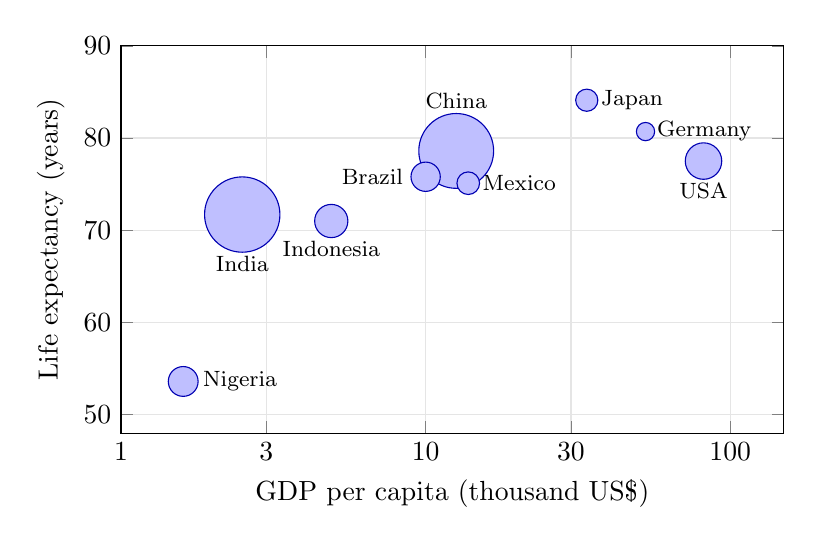
\begin{tikzpicture}[country/.style={font=\footnotesize, inner sep=1pt}]
  \begin{semilogxaxis}[
    width=10cm, height=6.5cm, xmin=1, xmax=150, ymin=48, ymax=90,
    xtick={1,3,10,30,100}, xticklabels={1, 3, 10, 30, 100},
    xlabel={GDP per capita (thousand US\$)}, ylabel={Life expectancy (years)},
    grid=major, grid style={gray!20}
  ]
    % Mark size is a radius, so it goes with the square root of the population (millions) for the area to match it.
    \addplot[scatter, only marks, mark=*, scatter/use mapped color={draw=blue!70!black, fill=blue!25},
      visualization depends on={0.36*sqrt(\thisrow{pop}) \as \r},
      scatter/@pre marker code/.append style={/tikz/mark size=\r, /tikz/fill opacity=0.7},
    ] table {
      gdp   life  pop
      81.7  77.5  335
      33.8  84.1  124
      52.7  80.7  84
      12.6  78.6  1410
      13.8  75.1  129
      10.0  75.8  216
      4.9   71.0  278
      2.5   71.7  1429
      1.6   53.6  224
    };
    \node[country, below=7pt] at (axis cs:81.7,77.5) {USA};
    \node[country, right=4pt] at (axis cs:33.8,84.1) {Japan};
    \node[country, right=3pt] at (axis cs:52.7,80.7) {Germany};
    \node[country, above=14pt] at (axis cs:12.6,78.6) {China};
    \node[country, right=4pt] at (axis cs:13.8,75.1) {Mexico};
    \node[country, left=7pt] at (axis cs:10.0,75.8) {Brazil};
    \node[country, below=6pt] at (axis cs:4.9,71.0) {Indonesia};
    \node[country, below=14pt] at (axis cs:2.5,71.7) {India};
    \node[country, right=6pt] at (axis cs:1.6,53.6) {Nigeria};
  \end{semilogxaxis}
\end{tikzpicture}
